\documentclass[12pt]{article}

% PACKAGES

\usepackage[
top=2.50cm,
bottom=2.50cm,
left=2cm,
right=2cm,
marginparsep=0pt,
marginparwidth=0pt]{geometry}
\usepackage{fancyhdr}
\usepackage{float}
\usepackage{cancel}
\usepackage{mathtools}
\usepackage{amsmath}
\usepackage{amsthm}
\usepackage{amssymb}
\usepackage{textcomp}
\usepackage{ulem}
\usepackage{verbatim}
\usepackage{contour}
\usepackage{graphicx}
\usepackage{svg}
\usepackage{xcolor}
\usepackage[T1]{fontenc}
\usepackage{inputenc}
\usepackage[utf8]{inputenx}
\usepackage[unicode]{hyperref}
\usepackage[shortlabels]{enumitem}
\usepackage{listings}
\usepackage{xcolor}
\usepackage{tocloft}
\usepackage{tikz}
\usepackage{xspace}
\usepackage[most]{tcolorbox}
\usepackage{pgf}
\usepackage{pgf-pie}

% MACROS & DEFS

\newcommand{\modelmapper}{\texttt{modelmapper}\xspace}

\newcommand{\note}[1]{\textbf{Note:} #1}

\newcommand{\floor}[1]{\left\lfloor #1 \right\rfloor}
\newcommand{\ceil}[1]{\left\lceil #1 \right\rceil}
\newcommand{\round}[1]{\left\lfloor #1 \right\rceil}
\newcommand{\abs}[1]{\left\lvert #1 \right\rvert}

\DeclareRobustCommand{\ul}[1]{%
	\uline{\phantom{#1}}%
	\llap{\contour{white}{#1}}%
}

\renewcommand{\ULdepth}{1.8pt}
\contourlength{0.8pt}

\setlength{\parindent}{0em}
\setlength{\parskip}{0.75em}

\definecolor{codegreen}{RGB}{0,135,0}
\definecolor{codegray}{RGB}{135,135,135}
\definecolor{codemagenta}{RGB}{215,0,135}
\definecolor{codepurple}{RGB}{135,0,175}
\definecolor{backcolour}{RGB}{238,238,238}

\definecolor{bookyellow}{RGB}{255,255,224}

\DeclareTotalTCBox{\shell}{ O{black} v !O{} }
{
    fontupper=\ttfamily,
    nobeforeafter,
    tcbox raise base,
    arc=0pt,
    outer arc=0pt,
    top=0.1mm,
    bottom=0.1mm,
    left=0.1mm,
    right=0.1mm,
    leftrule=0pt,
    rightrule=0pt,
    toprule=0.3mm,
    bottomrule=0.3mm,
    boxsep=0.5mm,
    colback=#1!60!white,
    colframe=#1!70!black,
    #3
}{\textcolor{white}{#2}}

% PACKAGE CONFIG

\lstdefinestyle{code}{
	basicstyle=\ttfamily\small,
	commentstyle=\color{codegray}\itshape,
	keywordstyle=\color{codepurple},
	stringstyle=\color{codegreen},
	aboveskip=25pt,
    belowskip=10pt,
	captionpos=b,
	abovecaptionskip=12.5pt,
	breaklines=true,
	numbers=none,
	frame=tb,
	framesep=5pt,
	keepspaces=true,
	showspaces=false,
	showstringspaces=false,
	breakatwhitespace=false,
	tabsize=2,
	showtabs=false,
}

\lstset{style=code}

% Set dots for table of contents
\renewcommand{\cftdot}{.}
\renewcommand{\cftsecleader}{\cftdotfill{\cftdotsep}}

% Set theorem
\newtheorem*{definition}{Definition}

% HEADER & FOOTER

\setlength{\headheight}{15pt}
\pagestyle{fancy}
\renewcommand{\headrulewidth}{0pt}
\lhead{J. Scerri}
\chead{CPS2002 --- Code Analysis}
\rhead{\thepage}

% TITLE

\title{CPS2002 --- Code Analysis\\
\vspace{1em}\textbf{Assignment Part 2}}

\date{\today}

\author {{\textbf{Juan Scerri}}\\
B.Sc. (Hons)(Melit.) Computing Science and Mathematics (Second Year)}

\begin{document}

%----------------------------------
%	TITLE PAGE
%----------------------------------

\maketitle % Print the title page

\thispagestyle{empty} % Suppress headers and footers on the title page

%----------------------------------

\tableofcontents

\clearpage

\listoffigures

\lstlistoflistings

\clearpage

\section{Plagiarism Declaration}

Plagiarism is defined as \textit{``the unacknowledged use, as
one's own, of work of another person, whether or not such work
has been published, and as may be further elaborated in Faculty
or University guidelines''} (\ul{University Assessment
Regulations}, 2009, Regulation 39 (b)(i), University of Malta).

I, the undersigned, declare that the report submitted is my
work, except where acknowledged and referenced. I understand
that the penalties for committing a breach of the regulations
include loss of marks; cancellation of examination results;
enforced suspension of studies; or expulsion from the degree
programme.

Work submitted without this signed declaration will not be
corrected, and will be given zero marks.

\vfill

\begin{minipage}[t]{0.3\textwidth}
\ul{Juan Scerri} \medskip

\textbf{Student's full name} \medskip
\end{minipage}
\hfill
\begin{minipage}[t]{0.3\textwidth}
\ul{CPS2002} \medskip

\textbf{Study-unit code} \medskip
\end{minipage}
\hfill
\begin{minipage}[t]{0.3\textwidth}
\ul{{\today}} \medskip

\textbf{Date of submission} \medskip
\end{minipage}

\vspace{2cm}

\textbf{Title of submitted work:} \ul{CPS2002 Code Analysis}

\vspace{2cm}

\textbf{Student's signature} \medskip

\underline{\includegraphics[height=2cm]{images/sig.png}} \medskip

\section{Selected Open--Source Project}

The selected open--source project which will be analysed in this
report is the \modelmapper project. It is a simple Java library
which allows for the conversion of a class into another (see
listing \ref{modelmapper-usage}).

\begin{lstlisting}[language=Java, caption={Using the
\modelmapper library}, label={modelmapper-usage}]
public class PersonEntity {
    public Id id;
    public String name;
    public String surname;
    public int age;

    // getter and setters
}

public class Person {
    public Id id;
    public String name;
    public String surname;
    public int age;

    // getter and setters
}

Person person = (new ModelMapper()).map(personEntity, Person.class);
\end{lstlisting}

At the time of writing the project has $721$ commits, $220$ open
issues and $11$ open pull requests. The project was clone from
GitHub and since the project uses Maven, the test suite was ran
with the command \shell{mvn clean test}, (see figure
\ref{running-test-suite}).

Furthermore, the test suite was run from within IntelliJ to get
code coverage metrics (see figure \ref{intellij-code-coverage}).

% The overall line coverage of the project was $82\%$. This is a
% significant amount of the code and hence the project is being
% sufficiently tested with regards to all possible code paths.
%
% Nevertheless, this is \textbf{not} a guarantee of the project.
% This is because certain tests can have artificially high code
% coverage whilst only really testing a small subset of the
% covered area. This is very common when unit tests call
% high--level methods to test the library/application.

\begin{figure}[H]
    \centering
    \includegraphics[width=14cm]{images/test-suite.png}
    \caption{Running the test suite from the terminal}
    \label{running-test-suite}
\end{figure}

\begin{figure}[H]
    \centering
    \includegraphics[width=14cm]{images/code-coverage.png}
    \caption{Code coverage metrics generated by IntelliJ}
    \label{intellij-code-coverage}
\end{figure}

Additionally, object-oriented data about the project was
extracted using CodeMR.

\begin{figure}[H]
    \centering
    \includegraphics[height=12cm]{images/codemr-metrics.png}
    \caption{HTML report generate by CodeMR for the \modelmapper
    module}
    \label{codemr-metrics}
\end{figure}

\section{Project Analysis}

\subsection{Object--Oriented Metrics}

\subsubsection{Complexity}

\begin{figure}[H]
    \centering
    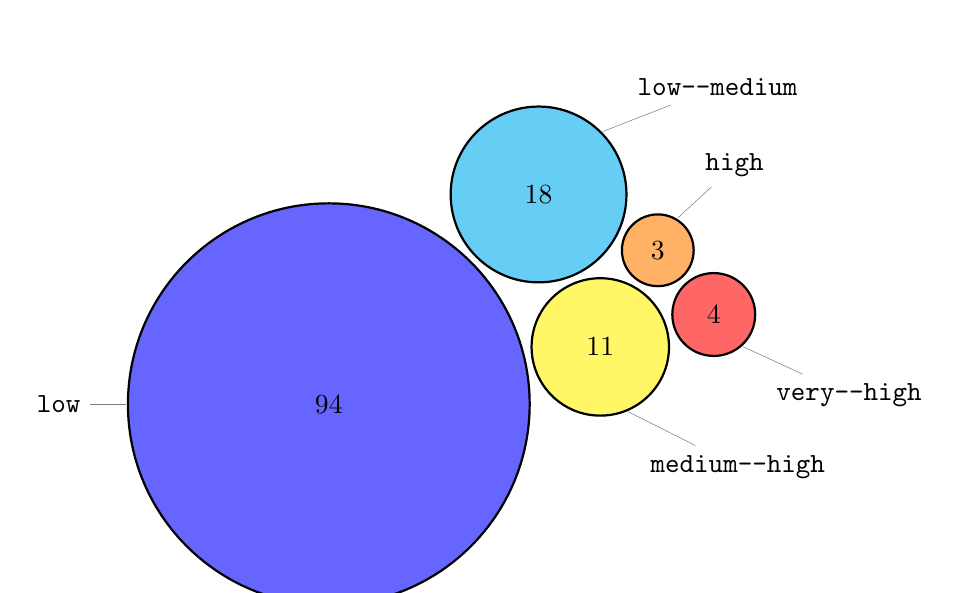
\begin{tikzpicture}
        \pie[sum=auto, cloud, text=pin]{
            94/\texttt{low},
            18/\texttt{low--medium},
            11/\texttt{medium--high},
            3/\texttt{high},
            4/\texttt{very--high}
        }
    \end{tikzpicture}
    \caption{Number of classes which have \texttt{low} to
    \texttt{very--high} complexity}
\end{figure}

\note{The percentage values provided by CodeMR where not used.
This is because when converting from percentages to quantities
the values where not identical to the ones reported by CodeMR.}

CodeMR defines code complexity in the following way.

\begin{definition}
    A class is said to be \ul{complex} if it is difficult to
    understand and describes the interactions between a number
    of entities. Higher levels of complexity increase the risk
    of unintentionally interfering with interactions and so
    increases the chance of introducing defects when making
    changes.
\end{definition}

CodeMR reports that only $7$ classes have a \texttt{high} or
\texttt{very--high} complexity. However, this does not mean that
the project is not complex.

Apart from the complexity brought on by \textbf{branching} as
mentioned in McCabe's Cyclomatic Complexity, there are other
factors. Specifically, \textbf{indirection} caused by dependency
injection or function calls also adds complexity as the
programmer has to jump from one segment of code to another to
understand.

\begin{figure}[H]
    \centering
    \includegraphics[width=14cm]{images/problematic-classes.png}
    \caption{A list of problematic classes identified by CodeMR}
    \label{problematic-classes}
\end{figure}

\begin{lstlisting}[language=Java,label={internal-method},caption={An
internal method in the class \texttt{TypeMapImpl} which
was reported by CodeMR as having \texttt{very--high}
complexity}]
@Override
public <P> TypeMap<S, D> include(TypeSafeSourceGetter<S, P> sourceGetter, Class<P> propertyType) {
  @SuppressWarnings("unchecked")
  TypeMapImpl<? super S, ? super D> childTypeMap = (TypeMapImpl<? super S, ? super D>)
      configuration.typeMapStore.get(propertyType, destinationType, name);
  Assert.notNull(childTypeMap, "Cannot find child TypeMap");

  List<Accessor> accessors = PropertyReferenceCollector.collect(this, sourceGetter);
  for (Mapping mapping : childTypeMap.getMappings()) {
    InternalMapping internalMapping = (InternalMapping) mapping;
    addMapping(internalMapping.createMergedCopy(accessors, Collections.<PropertyInfo>emptyList()));
  }
  return this;
}
\end{lstlisting}

Furthermore, additional barriers to understanding this
particular project are: extensive use of \textbf{unchecked
code}, \textbf{reflection} and \textbf{generics} (see listing
\ref{internal-method}). Unfortunately, Java has limited
capabilities when it comes to reflection and generics requiring
the use of unchecked code.

This naturally makes the project for any observer highly
complex. However, after acquainting one's self with the
terminology used and the less complex classes in the project it
will overall be easier to understand the more complicated pieces
of code. So, from that perspective overall the project has a
\texttt{medium} complexity given that it is solving quite a
complicated problem. 

\subsubsection{Coupling}

\begin{figure}[H]
    \centering
    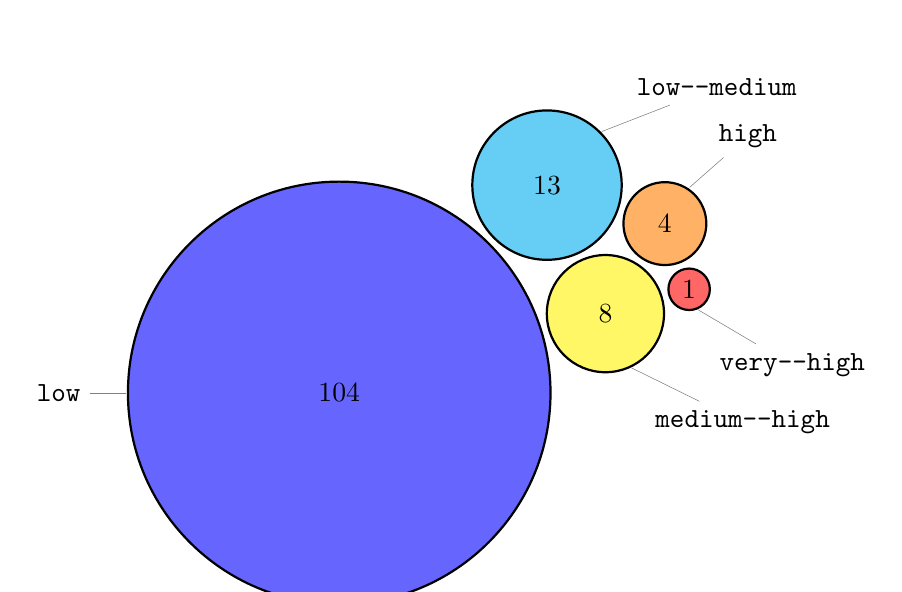
\begin{tikzpicture}
        \pie[sum=auto, text=pin, cloud]{
            104/\texttt{low},
            13/\texttt{low--medium},
            8/\texttt{medium--high},
            4/\texttt{high},
            1/\texttt{very--high}
        }
    \end{tikzpicture}
    \caption{Number of classes which have \texttt{low} to
    \texttt{very--high} coupling}
\end{figure}

\begin{definition}
    Two classes \textbf{A} and \textbf{B} are \ul{coupled} if:
    \begin{itemize}
        \item \textbf{A} has an attribute that refers to (is of type)
            \textbf{B}.
        \item \textbf{A} calls on services of an object
            \textbf{B}.
        \item \textbf{A} has a method that references \textbf{B}
            (via return type or parameter).
        \item \textbf{A} has a local variable which type is
            class \textbf{B}.
        \item \textbf{A} is a subclass of (or implements) class
            \textbf{B}.
    \end{itemize}

    Furthermore, tightly coupled systems tend to exhibit the
    following characteristics:
    \begin{itemize}
        \item A change in a class usually forces a ripple effect
            of changes in other classes.
        \item Requires more effort and/or times due to the
            increased dependency.
        \item Might be harder to reuse a class because
            dependency classes must be included.
    \end{itemize}

\end{definition}

\subsection{Test Suite Suitability}

\subsection{Maintainability}

\end{document}
